%
% ─── CAPITULO 6: VISUALIZACION DE FRACTALES 2D ──────────────────────────────────
%

En el capítulo \ref{chap:renderizacion} introdujimos el uso de WebGL como herramienta de renderizado de imágenes y estudiamos sus componentes, sin embargo, no olvidemos que nuestro objetivo es la visualización de fractales, donde la característica principal de los mismos es que no se pueden expresar a partir de un conjunto de vértices o líneas, sino que son curvas o superficies totalmente irregulares. Por tanto, a efectos prácticos, nuestro vertex shader tomará como entrada los vértices $(-1,-1)$, $(1,-1)$, $(1,1)$ y $(-1,1)$ y no aplicará ninguna transformación, pues ya están normalizados en el clip space (teniendo en cuenta que estaríamos visualizando un fragmento del plano $z=0$). Cabe en este momento aclarar que en el ámbito de herramientas de renderizado se utiliza el convenio de utilizar la coordenada $Y$ para la altura y la coordenada $Z$ para la profundidad. 

A partir de estos cuatro vértices, en el canvas se visualizarán dos triángulos que completarán la superficie completa del mismo. El vertex shader a partir de ahora será totalmente trivial, pues solo devolverá en la variable \verb|gl_Position| la misma posición que obtiene del buffer de posición.

\begin{lstlisting}
attribute vec2 a_Position;
void main() {
    gl_Position = vec4(a_Position.x, a_Position.y, 0.0, 1.0);
}
\end{lstlisting}

Mientras que, por su parte, el fragment shader podrá acceder a la posición (en coordenadas de dispositivo) del píxel que se está ejecutando mediante la variable \verb|gl_FragCoord| y a partir de estas coordenadas devolver un color en la variable \verb|gl_FragColor|. Es decir, estamos dibujando una escena completa, próximamente un fractal, en dos triángulos. Por ejemplo, las imágenes \ref{fig:julia-intro} y \ref{fig:mandelbrot-intro} son el resultado de esta metodología. 

\section{Objetivo}

Procedemos a explicar el objetivo principal de este objetivo y para el cual programaremos cada línea de código: Queremos desarrollar una página web interactiva, que cuente con un canvas donde se renderice el fractal que deseemos y, además, haya una serie de parámetros que se puedan controlar dinámicamente, de forma que conforme se cambia un parámetro el canvas modifica la imagen que está renderizando.

Queremos visualizar conjuntos de Julia $\mathcal{J}_c$ para distintos $c\in\C$, el conjunto de Mandelbrot, y las generalizaciones de los conjuntos de Julia y Mandelbrot ocasionadas si se itera la función $P_{c,N}(z)=z^N+c$ para distintos valores de $N\in\N$. Además, si revisitamos el algoritmo que utilizamos en la sección \ref{subsection:representacion-julia} para graficar en \textit{Mathematica} conjuntos de Julia y el que utilizamos en la sección \ref{subsection:representacion-mandelbrot} para visualizar el conjunto de Mandelbrot, podremos recordar que para aproximar qué puntos del plano complejo eran prisioneros o de escape fijábamos un número máximo de iteraciones $M$, tras las cuales se consideraba que un número $z_0\in\C$ era prisionero si la sucesión de los módulos de sus iteradas $\{P_{c,N}^n(z_0)\}$ no superaba el número de escape $e_c=\max\{2,|c|\}$ . Este valor $M$ también podría ser un parámetro modificable, para así poder ver dinámicamente cómo cambia la resolución cuando se cambia el número máximo de iteraciones.

Además, conviene añadir la posibilidad de desplazarse y hacer zoom en distintas regiones del plano, para así poder explorar en detalle las regiones del fractal, permitiendo observar en detalle las autosimilaridades que nos ofrecen, como ya vimos en la sección \ref{section:autosimilaridad-julia-mandelbrot}. 


\section{Estructurando el código}
\label{section:codigo}

Podemos usar como base el código utilizado para visualizar el cuadrado de colores, ya que nos puede venir bien su estructura para adaptar la misma a la renderización de fractales. Sin embargo, tiene una estructura muy procedural. Podemos mantener la misma arquitectura de forma que cambiando los elementos que sean necesarios y el código de los shaders podamos ver los fractales que deseemos, pero en ese caso la depuración se complicaría, el código es más difícil de leer y cuesta mucho añadir interactividad. Por este motivo, adaptaremos el código a un paradigma orientado a objetos, modularizando los distintos componentes, creando abstracciones de las herramientas que proporciona WebGL y siguiendo los \href{https://medium.com/backticks-tildes/the-s-o-l-i-d-principles-in-pictures-b34ce2f1e898}{principios SOLID}.

En concreto, para el código de JavaScript hemos creado las siguientes clases:
\begin{itemize}
    \item \verb|Scene2D|: Inicializa y gestiona todos los componentes de WebGL necesarios para renderizar una escena: el contexto WebGL, los parámetros, el shader, las variables del shader y los buffers. Cuenta además con métodos getter y setters de cada uno de los parámetros de la escena y un método \verb|draw| que renderiza la escena a partir de los parámetros actuales.
    \item \verb|ShaderType|: Es un enumerado que puede tomar los valores \verb|ShaderType.vertexShader| o \verb|ShaderType.fragmentShader|
    \item \verb|Shader|: Representa una abstracción de lo que sería un `vertex shader' o un `fragment shader'. A partir del código fuente y del tipo de shader, se compila y almacena el shader en un atributo.
    \item \verb|ShaderProgram|: A partir de dos objetos de la clase \verb|Shader|, que serían el vertex shader y el fragment shader, crea el programa shader final.
    \item \verb|Buffer|: Construye un buffer de WebGL a partir de un array de JavaScript que se le pasa como parámetro.
\end{itemize}

Además, el fichero \verb|fractals-2D.js| utiliza un objeto de la clase \verb|Scene2D| para interactuar con el DOM, gestionar los eventos y así poder modificar dinámicamente los parámetros, de tal forma que cada vez que se interactúa con la página se registra un evento con una función manejadora asociada. Esta función manejadora utiliza los setters correspondientes del objeto \verb|Scene2D| y hace las modificaciones correspondientes para finalmente llamar a \verb|draw| y así modificar dinámicamente la visualización.

El código completo se puede encontrar en GitHub: \url{https://github.com/JAntonioVR/Geometria-Fractal/tree/main/static}. La funcionalidad completa y detallada de cada clase puede consultarse en el apéndice \ref{appendix:javascript}.

\section{El fragment shader}
\label{section:fs-2D}

Como dijimos al inicio de este capítulo, nuestro vertex shader es trivial, simplemente asigna a \verb|gl_Position| las mismas coordenadas que se introducen desde JavaScript al buffer de posiciones. Es en el fragment shader donde se realiza el grueso de la programación necesaria para poder visualizar los distintos fractales.

Recordemos que el fragment shader se ejecuta una vez por cada píxel, de manera que podemos identificar la superficie completa del canvas con una región $[x_1,x_2]\times [y_1,y_2]\subseteq\R^2\cong\C$ del plano complejo y en particular cada píxel con un número complejo. Para ello, necesitamos transformar las coordenadas de dispositivo que el shader encuentra en la variable \verb|gl_FragCoord|. Supongamos que queremos inicialmente visualizar la región $[-2,2]\times[-2,2]$ y que las coordenadas de dispositivo son $(x,y)\in[0,720]\times[0,720]$, las cuales están precisamente en la región $[0,720]\times[0,720]$ porque las dimensiones del canvas son $720\times 720$ píxeles. Entonces la transformación lineal que necesitamos es 
\begin{equation}
\label{eq:transformacion-lineal-1}
\begin{split}
    \phi:[0,720]\times[0,720] & \longrightarrow [-2,2]\times[-2,2] \\
    (x,y) & \longmapsto \frac{4}{720}(x,y)-(2,2)
\end{split}
\end{equation}

De esta forma, a partir de las coordenadas de dispositivo obtenemos un punto del plano complejo. Supongamos ahora que en lugar de querer visualizar la región $[-2,2]\times[-2,2]$ queremos representar cualquier otra, pero aún centrada en el origen $(0,0)$. Podemos generalizar la transformación $\phi$ para cualquier otro intervalo, pero en lugar de ello y para mantener las proporciones introduciremos una variable que represente el \textit{zoom} que se aplica a la imagen, de tal forma que tan solo habría que multiplicar el resultado de la transformación por una constante $\lambda$. Esta constante será menor que $1$ si se desea acercar la región o mayor que $1$ si se desea alejar. Por tanto la nueva transformación será

\begin{equation}
    \label{eq:transformacion-lineal-2}
    \begin{split}
        \phi:[0,720]\times[0,720] & \longrightarrow [-2,2]\times[-2,2] \\
        (x,y) & \longmapsto \lambda\left(\frac{4}{720}(x,y)-(2,2)\right)
    \end{split}
\end{equation}

Y por último, procedemos a buscar la forma de representar cualquier parte del plano centrada o no. Tenemos entonces que fijar un par $(x_0,y_0)$ que sea el centro de la región en la que se hace este posible zoom, que hasta este momento hemos asumido que es el $(0,0)$, pero a partir de ahora queremos que tome cualquier valor. Aprovechando que la transformación (\ref{eq:transformacion-lineal-2}) nos devuelve coordenadas en regiones centradas simplemente tenemos que sumar este par al resultado, de forma que nos queda 

\begin{equation}
    \label{eq:transformacion-lineal-3}
    \begin{split}
        \phi:[0,720]\times[0,720] & \longrightarrow [-2,2]\times[-2,2] \\
        (x,y) & \longmapsto (x_0,y_0) + \lambda\left(\frac{4}{720}(x,y)-(2,2)\right)
    \end{split}
\end{equation}
donde las constantes de zoom $\lambda$ y el centro $(x_0,y_0)$ pueden ser parametrizables para así poder visualizar cualquier región del plano en el canvas. La forma de darle distintos valores a estas constantes es mediante una variable \verb|uniform| para cada caso, de forma que queda el siguiente fragmento de código:

\begin{lstlisting}
// Zoom: constante lambda que define el tamano de la region a representar
uniform float u_zoomSize;
// Zoom center: Punto del plano situado en el centro del canvas
uniform vec2 u_zoomCenter;

// ... 

vec2 get_world_coordinates() {
    // Coordenadas de dispositivo normalizadas en [0,1]x[0,1]
    vec2 uv = gl_FragCoord.xy / vec2(720.0, 720.0);
    // Punto del plano complejo al que corresponde el pixel
    return u_zoomCenter + (uv * 4.0 - vec2(2.0)) * u_zoomSize;
}
\end{lstlisting}

Y ya tenemos en el shader una función que calcula el punto del plano al cual corresponde el píxel. A partir de esto, y al igual que en el capítulo \ref{chap:Julia-Mandelbrot}, tan solo tenemos que iterar la función $P_{c,N}$ y en función del número de iteraciones necesarias para diverger (o no), asignar un color.

\subsection{La función $f(z)=z^N+c$}

Necesitamos código para la función $P_{c,N}$, pero esta requiere a su vez la programación de potencias de números complejos. Tal y como se ha evidenciado en el código recientemente presentado, y de manera natural, representaremos un número complejo $z=x+i\cdot y\cong (x,y)\in\R^2$ mediante una variable del tipo \verb|vec2|. Por lo que debemos implementar una función que, de forma iterativa, multiplique (usando el producto de números complejos) $N$ veces por sí mismo una variable \verb|vec2|. Como ya sabemos,
$$
z^2 = (\Re z+i\cdot \Im z)(\Re z+i\cdot \Im z) = ((\Re z)^2-(\Im z)^2) + 2\cdot\Re z\cdot\Im z\cdot i
$$

y como $z^n = z^{n-1}\cdot z$, entonces

\begin{equation}
    \label{eq:potencias-complejos}
    \begin{split}
        z^n & = z^{n-1}\cdot z = (\Re z^{n-1} + \Im z^{n-1}\cdot i)\cdot(\Re z + \Im z\cdot i) \\
        & = \left(\Re z^{n-1}\cdot\Re z - \Im z^{n-1}\cdot \Im z\right) + \left(\Re z^{n-1}\cdot\Im z + \Im z^{n-1}\cdot\Re z\right)\cdot i 
    \end{split}
\end{equation}
y esto es válido para cualquier $n\in\N$. Podemos utilizar iterativamente la ecuación (\ref{eq:potencias-complejos}) para programar un método que calcule potencias complejas:
\begin{lstlisting}
// Potencias complejas
vec2 complex_pow(vec2 z, int n) {
    vec2 current_pow = vec2(1.0, 0.0);
    for (int i = 1; i < 100; i++) {
        vec2 z_ant = current_pow;
        current_pow = vec2( z_ant.x*z.x - z_ant.y*z.y, 
                            z_ant.x*z.y + z_ant.y*z.x);
        if(i >= n) break;
    }
    return current_pow;
}
\end{lstlisting}

Recordamos, para el que no esté acostumbrado al código GLSL, que este lenguaje no permite iterar bucles utilizando variables, por lo que necesitamos fijar un máximo de iteraciones (en este caso 100) y salir del bucle al alcanzar las \verb|n| iteraciones.

Una vez tenemos esta función, es muy sencillo programar la función $P_{c,N}$ aprovechando la aritmética preprogramada para los objetos vector en GLSL.

\begin{lstlisting}
vec2 P(vec2 z, vec2 c, int n) {
	return complex_pow(z,n) + c;
}
\end{lstlisting}

En el caso de los conjuntos de Julia debemos fijar una constante $c$ a la cual calcularle el conjunto $\mathcal{J}_c$. Naturalmente esta constante es común a todos los píxeles, por lo que necesitamos una variable \verb|uniform| para desde JavaScript enviar al shader qué conjunto de Julia queremos graficar. Además, también debemos fijar el exponente $N$ que también es común a todos los píxeles, por lo que hacemos uso de otra variable \verb|uniform| al uso.

\begin{lstlisting}
// Valor c fijo en la funcion z^N + c
uniform vec2 u_juliaSetConstant;
// Valor N fijo en la funcion z^N +c
uniform int u_order;
\end{lstlisting}

\subsection{Asignación de colores}
\label{subsection:colores}

Con la función $P_{c,N}$ ya programada, recordamos los algoritmos que utilizamos en \textit{Mathematica} para graficar conjuntos de Julia y Mandelbrot, reprogramándolos ahora en GLSL para poder renderizar dichos conjuntos. Estos consistían en iterar la función $P_{c,N}$, cada uno a su manera, fijando un número máximo de iteraciones $M$ tras las cuales se decidía qué puntos son prisioneros o de escape y almacenando en una variable cuántas iteraciones se han necesitado para tomar esta decisión. En función del valor de dicha variable asignamos un color. Por tanto, necesitamos una forma de, a partir de este valor, asignar un color.

Lo primero de todo, este número máximo de iteraciones $M$ es clave en esta asignación de colores. Queremos además que sea parametrizable, por lo que declaramos en el shader una variable \verb|uniform| cuyo valor le pasaremos al shader con JavaScript.

\begin{lstlisting}
// Numero de iteraciones maximo para decidir que elementos son
// prisioneros o escapan
uniform int u_maxIterations;
\end{lstlisting}

Seguidamente diseñaremos una paleta de colores y mediante interpolación lineal calcularemos qué color asignar a cada píxel. Podemos tomar tantos colores como queramos y elegir qué colores. Tras varias pruebas hemos decidido asignar el color negro (\verb|rgb(0, 0, 0)=#000000|) para los puntos prisioneros (los que no divergen tras las $M$ iteraciones) y para los que escapan utilizar un gradiente entre los siguientes colores:

\begin{figure} [ht]
    \centering
    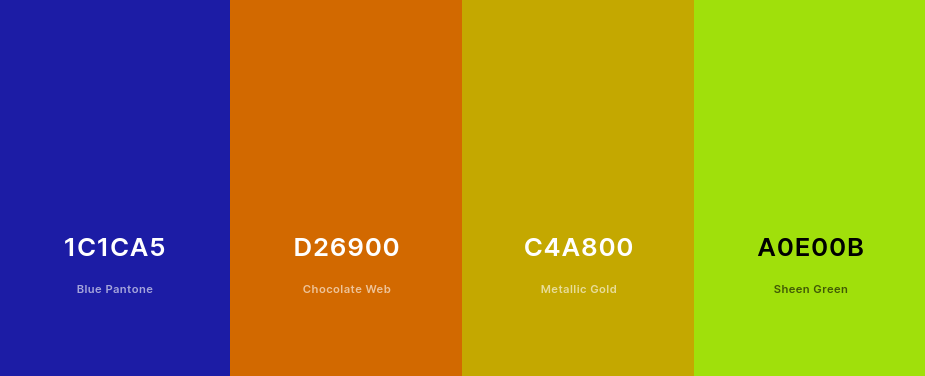
\includegraphics[scale = 0.4]{img/C6/paleta.png}
    \caption{Paleta de colores elegida para la visualización de fractales 2D}
    \label{fig:paleta}
\end{figure}

La cual nos proporciona el siguiente gradiente, que proximamente podremos ver en nuestros fractales, de manera que los puntos que diverjan antes se acercarán más al azul y los que tarden más se colorearán de un color más parecido al verde.

\begin{figure} [ht]
    \centering
    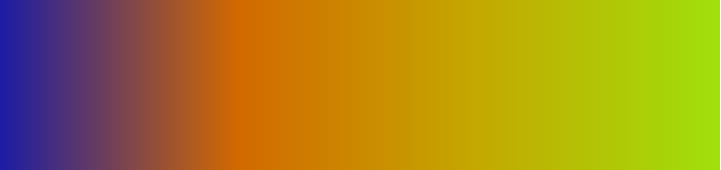
\includegraphics[scale = 0.51]{img/C6/gradiente.png}
    \caption{Gradiente generado por la paleta de colores \ref{fig:paleta}}
    \label{fig:gradiente}
\end{figure}

Con esta decisión tomada, presentamos el código utilizado

\begin{lstlisting}
// Paleta de colores, a partir de un numero 0<=t<=1 y 4 
// colores c1, c2, c3 y c4 devuelve el color 
// correspondiente en el gradiente creado por los cuatro 
// colores.
vec3 palette(float t, vec3 c1, vec3 c2, vec3 c3, vec3 c4) {
    float x = 1.0 / 3.0;
    if (t < x) return mix(c1, c2, t/x);
    else if (t < 2.0 * x) return mix(c2, c3, (t - x)/x);
    else if (t < 3.0 * x) return mix(c3, c4, (t - 2.0*x)/x);
    return c4;
}

// Asignacion de colores, a partir de una variable que define
// si el punto es prisionero o de escape y el numero de 
// iteraciones antes de escapar se asigna a la variable 
// gl_FragColor el color que le corresponde.
void assignColor(bool escaped, int iterations) {
    gl_FragColor = escaped ? vec4(palette(
      3.0*float(iterations)/ float(u_maxIterations),
      vec3(0.109, 0.109, 0.647), // #1C1CA5
      vec3(0.823, 0.411,   0.0), // #D26900
      vec3(0.769, 0.659,   0.0), // #C4A800
      vec3(0.627, 0.878, 0.043)  // #A0E00B
      ), 
      1.0) : vec4(vec3(0.0,0.0,0.0), 1.0);
}
\end{lstlisting}

Como se puede observar, es una simple interpolación lineal entre los 4 colores que se acaban de presentar, que en GLSL deben codificarse como tripletas RGB donde cada componente está normalizada entre 0 y 1.

\subsection{Renderizando conjuntos de Julia}
\label{subsection:render-julia}

Tenemos entonces todos los ingredientes para programar el renderizado, tan solo falta decidir si el punto que representa el píxel es prisionero o escapa mediante la iteración de $P_{c,N}$. Tras obtener las coordenadas de mundo que se le asignan al píxel mediante el método descrito al inicio de esta sección, debemos iterar la función $P_{c,N}$ almacenando el número de iteraciones dadas. Atendiendo al teorema \ref{th:escape}, en caso de que el módulo supere el valor 2 se decide que el punto es de escape. Si esto nunca ocurre y se alcanza el número máximo de iteraciones sin que el módulo sea mayor que 2, entonces se decide que el punto es prisionero. Atendiendo a esta decisión y al número de iteraciones dadas se asigna el color correspondiente como comentamos en la sección \ref{subsection:colores}. El código GLSL sería el siguiente:

\begin{lstlisting}
// A partir del valor de la constante c y el exponente n
// iteramos la funcion P_{c,N} y asignamos el color.
void Julia(vec2 c, int n) {
    vec2 z0 = get_world_coordinates();
    int iterations;
    vec2 z = z0;
    bool escaped = false;
    float length_c = length(c);
    for(int i = 0; i < 10000; i++) {
        if(i > u_maxIterations) break;
        iterations = i;
        z = P(z, c, n);
        if (length(z) > 2.0){
            escaped = true;
            break;
        }
    }

    assignColor(escaped, iterations);
}
\end{lstlisting}

Ya desde la función \verb|main|, llamamos a esta función recién presentada y obtenemos los resultados que se presentan en las imágenes \ref{fig:julia-webgl}.  

\begin{lstlisting}
Julia(u_juliaSetConstant, u_order);
\end{lstlisting}

\begin{figure}[ht]
    \centering
    \begin{tabular}{ccc}
      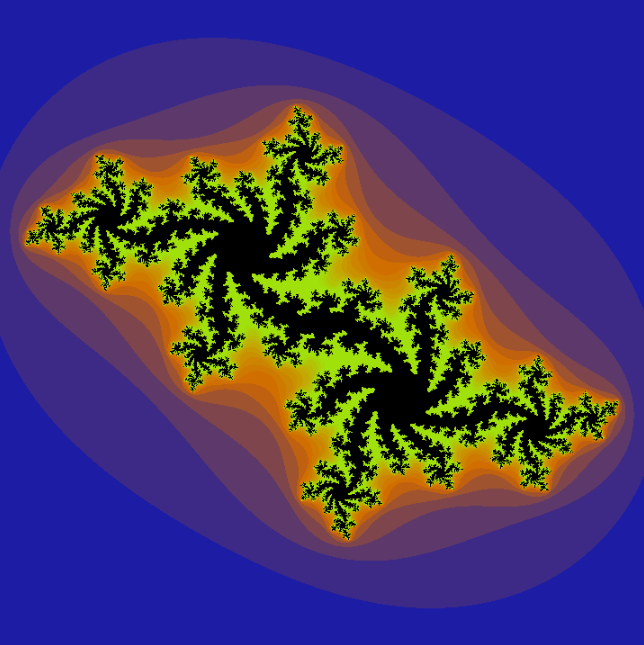
\includegraphics[scale=0.2]{img/C6/julia-1.png} &   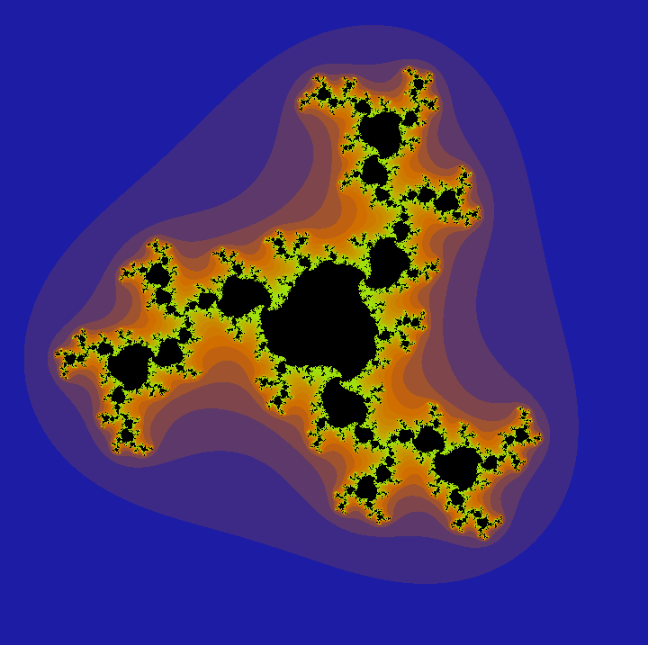
\includegraphics[scale=0.2]{img/C6/julia-2.png} &   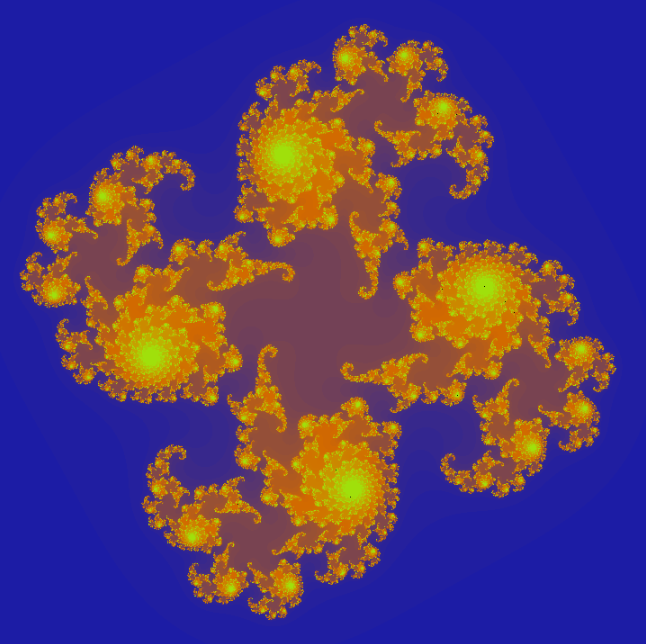
\includegraphics[scale=0.2]{img/C6/julia-3.png} \\
    (a) $z^2-0.38+0.62i$ & (b) $z^3+0.62+0.5i$ & (c) $z^4-0.24+0.5i$ \\[6pt]
    \end{tabular}
    \caption{Renderizado de algunos conjuntos de Julia con WebGL}
    \label{fig:julia-webgl}
\end{figure}

\subsection{Renderizando conjuntos de Mandelbrot}

Ya hemos visto la metodología a utilizar si queremos visualizar conjuntos de Julia y, como es de esperar, la metodología para graficar conjuntos de Mandelbrot $\mathcal{M}_N$ no es muy distinta. Recordamos que, tal y como afirmamos en las secciones \ref{section:Mandelbrot} y \ref{subsection:julia-mandelbrot-generalizados} el conjunto de Mandelbrot $\mathcal{M}_N$ se componía de aquellos elementos $c\in\C$ tales que el conjunto de Julia $\mathcal{J}_c$ es conexo, o equivalentemente, de aquellos cuya sucesión $\{P_{c,N}^n(0)\}$ no diverge.

La metodología consiste por tanto en obtener las coordenadas de mundo del píxel, iterar la función $P_{c,N}$ tomando $z_0=0$ como semilla y observar qué sucede. Por la proposición \ref{prop:mandelbrot-escape} afirmamos que en el momento que una iterada supere en módulo a 2, entonces la sucesión de iteradas es divergente. Por tanto, almacenamos en una variable el número de iteradas que se han calculado antes de que el módulo de la sucesión supere a 2 en caso de que lo haga. Si esto no ocurre, se etiqueta al punto como prisionero y por tanto el punto pertenece a $\mathcal{M}_N$. De nuevo, la forma de asignar un color al píxel depende de si la sucesión diverge o no y del número de iteraciones hasta decidir que diverge en dicho caso. El código GLSL por tanto es el siguiente:

\begin{lstlisting}
void Mandelbrot(int n) {
    vec2 c = get_world_coordinates();
    int iterations;
    vec2 z = vec2(0.0);
    bool escaped = false;
    for (int i = 0; i < 10000; i++) {
        if (i > u_maxIterations) break;
        iterations = i;
        z = P(z, c, n);
        if (length(z) > 2.0) {
            escaped = true;
            break;
        }
    }
    assignColor(escaped, iterations);    
}
\end{lstlisting}

Vemos que es muy parecida a la función \verb|Julia| presentada en la sección \ref{subsection:render-julia}. La diferencia fundamental se encuentra en que mientras en los conjuntos de Julia fijamos un $c\in\C$ y usamos el complejo asociado al píxel como semilla en el caso del conjunto de Mandelbrot usamos siempre $z_0=0$ como semilla y tomamos como $c$ el complejo que representa el píxel.

Por tanto, ya solo falta llamar a esta función desde \verb|main| y podremos ver el conjunto de Mandelbrot en detalle. Presentamos algunas imágenes de detalles del mismo, a la vez que animamos a revisitar las imágenes \ref{fig:mandelbrot-intro}, las cuales también se han obtenido mediante WebGL.

\begin{lstlisting}
Mandelbrot(u_order);
\end{lstlisting}

\begin{figure}[ht]
    \centering
    \begin{tabular}{ccc}
      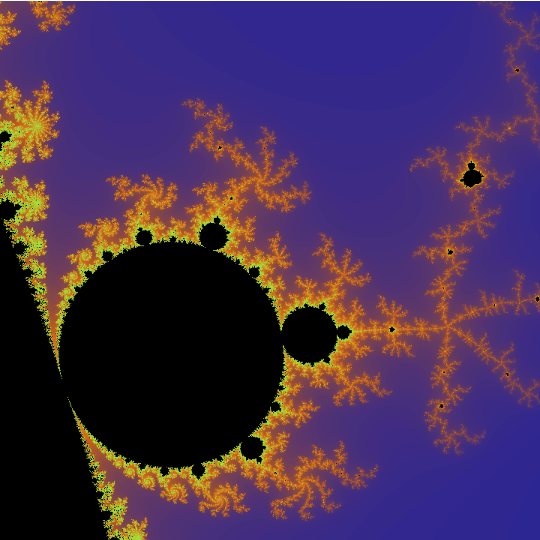
\includegraphics[scale=0.23]{img/C6/mandelbrot-1.png} &   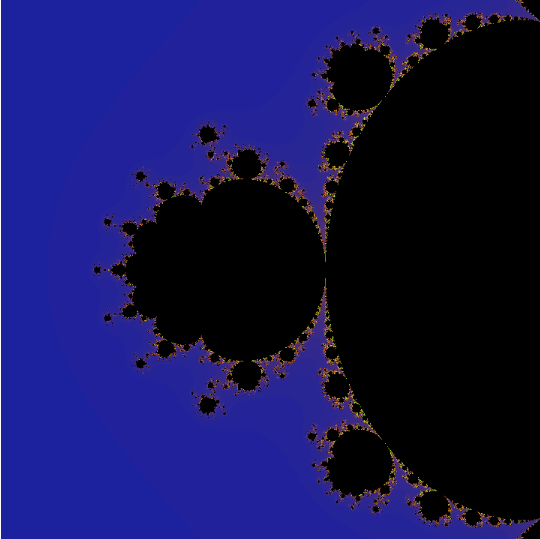
\includegraphics[scale=0.23]{img/C6/mandelbrot-2.png} &   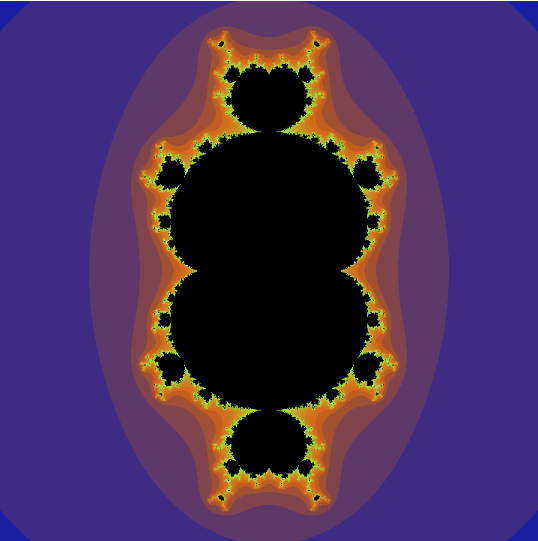
\includegraphics[scale=0.23]{img/C6/mandelbrot-3.png} \\
    (a) Detalle de $\mathcal{M}_2$ & (b) Detalle de $\mathcal{M}_8$ & (c) $\mathcal{M}_3$ \\[6pt]
    \end{tabular}
    \caption{Renderizado de algunos conjuntos de Mandelbrot con WebGL}
    \label{fig:mandelbrot-webgl}
\end{figure}

\subsection{Alternando conjuntos de Julia y Mandelbrot}

Finalmente, queremos dotar a nuestra web de la posibilidad de alternar qué fractal visualizar (Julia o Mandelbrot) y poder ajustar los parámetros a nuestro gusto. Para ello introducimos en el fragment Shader una variable \verb|uniform| entera que, en caso de valer 0 se visualizaría el conjunto de Mandelbrot y en caso de valer 1 se visualizaría el conjunto de Julia.

\begin{lstlisting}
// Renderizar conjunto de Julia o de Mandelbrot
uniform int u_fractal;

// ... 

void main() {
    if(u_fractal == 0)
        Mandelbrot(u_order);
    else
        Julia(u_juliaSetConstant, u_order);
}
\end{lstlisting}